\documentclass{examen}

\begin{document}
\modulo{Lenguajes de marcas y sistemas de gesti�n de informaci�n}


\pregunta{Una popular franquicia de cafeter�as desea ofrecer a sus clientes una aplicacion web para poder pedir su caf� de camino al trabajo.
Dados los siguientes requisitos y el HTML que se muestra, crear el fichero Javascript que consigue los resultados deseados}{10}

\begin{itemize}
\item{El usuario debe introducir su nombre  y los requisitos para preparar su caf�. Al final, en un {\tt div} con el {\tt id mensajes} aparecer� el texto ``Pepe, tu caf� costar� 2.40 euros''}
\item{Hay tres tipos de tama�o: corto (1.10 euros), largo (1.40) y extra-largo (1.90).}
\item{Se puede tener con leche (0.35 euros m�s) o sin leche (0 euros m�s).}
\item{Se puede pedir un extra de az�car (0.15 euros m�s) y con un vaso personalizado (0.80 euros m�s)}
\end{itemize}

Se debe tener en cuenta lo siguiente:
\begin{itemize}
\item{Se ha descubierto que determinadas combinaciones no parecer crear el tipo de sabor que caracteriza a la marca por lo que
no se permite que el usuario elija un caf� extra-largo sin leche pero con extra de az�car. Si ocurre esto se debe desmarcar todo y escribir un mensaje de error en el {\tt div} cuyo {\tt id} es {\tt errores}. Dicho mensaje debe llevar un fondo rojo creado desde Javascript}
\item{Est� permitido modificar el HTML.}
\item{Al cargar la p�gina no hay ning�n elemento marcado ni ning�n texto escrito.}
\end{itemize}

\break

\begin{figure}[h]
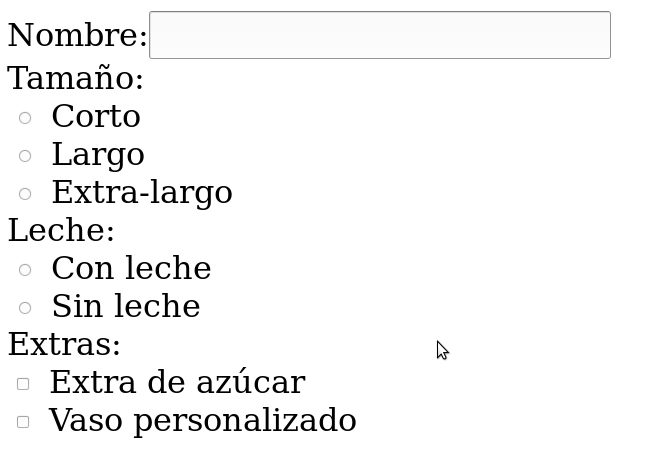
\includegraphics[scale=0.5]{examen-img/cafeteria.png}
\end{figure}
\begin{verbatim}
<!-- HTML con los controles-->
<form>
    Nombre:<input type="text" id="nombre"> <br/>
    Tama�o: <br/>
    <input type="radio" name="tamanio" id="corto"> Corto       <br/>
    <input type="radio" name="tamanio" id="largo"> Largo       <br/>
    <input type="radio" name="tamanio" id="extra"> Extra-largo <br/>
    Leche: <br/>
    <input type="radio" name="leche" id="con"> Con leche <br/>
    <input type="radio" name="leche" id="sin"> Sin leche <br/>
    Extras: <br/>
    <input type="checkbox" id="azucar"> Extra de az�car    <br/>
    <input type="checkbox" id="vaso"  > Vaso personalizado <br/>
</form>
<div id="errores"></div>
<div id="resultados"></div>
\end{verbatim}
\end{document}
